\section{Results}
\label{sec:results}

Table~\ref{tab:main} gives the main grid on Qwen2.5-1.5B for the six single-digit arithmetic targets and Table~\ref{tab:cap} the same grid for the three capital facts; Figure~\ref{fig:tradeoff} plots generalisation against neighbour damage per target. Every weight edit in these tables succeeds on the edited string unless the \emph{Exact} column says otherwise. Seed-to-seed variation is small compared with variation across targets (on the two targets run with three seeds, the median standard deviation over seeds of every rate in the table is 0 and the maximum is 0.06), so table entries average seeds within a target and then average targets; per-target points are shown in Figure~\ref{fig:tradeoff}.

\begin{table}[t]
\centering\small
\resizebox{\linewidth}{!}{\begin{tabular}{lrrrrrrrrrr}
\toprule
 & \multicolumn{3}{c}{should change? (edit / belief)} & \multicolumn{4}{c}{same domain, must not change} & \multicolumn{3}{c}{unrelated behaviour} \\
\cmidrule(lr){2-4}\cmidrule(lr){5-8}\cmidrule(lr){9-11}
Method & Exact & Para. & Entail. & Near chg. & (delayed) & Near KL & $\to$new & CF flip & Wiki KL & Chat KL \\
\midrule
In-context statement & 17 & 68 & 28 & 19 & 59 & 1.318 & 1 & -- & -- & -- \\
\addlinespace[2pt]
FT (1 string) & 100 & 39 & 6 & 30 & 71 & 2.096 & 16 & 0 & 2e-4 & 6e-5 \\
FT-L (1 MLP matrix) & 100 & 15 & 4 & 14 & 39 & 1.067 & 6 & 0 & 9e-5 & 6e-5 \\
LoRA (1 string) & 100 & 45 & 8 & 31 & 66 & 2.118 & 21 & 1 & 0.0014 & 5e-4 \\
ROME (operand token) & 100 & 73 & 21 & 23 & 31 & 1.176 & 3 & 0 & 1e-4 & 7e-4 \\
ROME (last token) & 67 & 57 & 21 & 56 & 87 & 2.712 & 17 & 1 & 1e-4 & 6e-4 \\
FT + paraphrases & 100 & 100 & 52 & 74 & 86 & 3.965 & 45 & 3 & 0.0040 & 0.0483 \\
\addlinespace[2pt]
FT + locality & 100 & 43 & 4 & 4 & 23 & 0.0258 & 1 & 1 & 6e-4 & 2e-4 \\
LoRA + locality & 100 & 31 & 3 & 3 & 10 & 0.0068 & 1 & 1 & 1e-3 & 6e-4 \\
\addlinespace[2pt]
FT string-keyed & 100 & 34 & 4 & 4 & 20 & 0.0333 & 1 & 1 & 6e-4 & 0.0054 \\
LoRA string-keyed & 100 & 21 & 1 & 3 & 12 & 0.0107 & 1 & 1 & 0.0011 & 0.0046 \\
\addlinespace[2pt]
FT proposition-keyed & 100 & 100 & 36 & 4 & 61 & 0.0147 & 4 & 1 & 0.0018 & 0.0727 \\
LoRA proposition-keyed & 100 & 97 & 35 & 1 & 52 & 0.0048 & 6 & 1 & 0.0036 & 0.0628 \\
\addlinespace[2pt]
FT prop.+consequences & 100 & 99 & 55 & 4 & 49 & 0.0150 & 3 & 1 & 0.0019 & 0.0623 \\
LoRA prop.+consequences & 100 & 98 & 58 & 1 & 42 & 0.0056 & 6 & 1 & 0.0037 & 0.0483 \\
\addlinespace[2pt]
SDF (LoRA, documents) & 100 & 89 & 36 & 4 & 23 & 0.0601 & 1 & 12 & 0.0562 & 0.0850 \\
SDF + locality & 0 & 63 & 24 & 3 & 17 & 0.0017 & 0 & 5 & 0.0096 & 0.0618 \\
\bottomrule
\end{tabular}
}
\caption{Arithmetic edits on Qwen2.5-1.5B-Instruct: mean over six single-digit targets (SDF rows: \edit{2+2=}{5} only). Rates in \%, KL in nats. Para./Entail.: held-out probes switched to the edit-consistent answer (forced choice). Near chg.: held-out neighbour probes answered correctly and immediately before the edit that are wrong after it. Near$\to$new: neighbours that now output the edit's new answer. Groups of rows: no weight change; unconstrained edits; one string with drift penalty; string-keyed; proposition-keyed; proposition and consequences; synthetic documents.}
\label{tab:main}
\end{table}

\begin{table}[t]
\centering\small
\resizebox{\linewidth}{!}{\begin{tabular}{lrrrrrrrrrr}
\toprule
 & \multicolumn{3}{c}{should change? (edit / belief)} & \multicolumn{4}{c}{same domain, must not change} & \multicolumn{3}{c}{unrelated behaviour} \\
\cmidrule(lr){2-4}\cmidrule(lr){5-8}\cmidrule(lr){9-11}
Method & Exact & Para. & Entail. & Near chg. & (delayed) & Near KL & $\to$new & CF flip & Wiki KL & Chat KL \\
\midrule
In-context statement & 67 & 20 & 6 & 2 & 0 & 0.440 & 0 & -- & -- & -- \\
\addlinespace[2pt]
FT (1 string) & 100 & 35 & 0 & 11 & 33 & 0.508 & 0 & 2 & 0.0011 & 3e-4 \\
FT-L (1 MLP matrix) & 100 & 26 & 0 & 14 & 100 & 0.846 & 0 & 4 & 0.0012 & 6e-4 \\
LoRA (1 string) & 100 & 46 & 7 & 22 & 100 & 0.938 & 0 & 6 & 0.0079 & 0.0014 \\
ROME (operand token) & 100 & 89 & 51 & 1 & 0 & 0.0502 & 0 & 1 & 3e-4 & 6e-4 \\
ROME (last token) & 100 & 39 & 4 & 25 & 100 & 2.763 & 0 & 5 & 2e-4 & 0.0019 \\
FT + paraphrases & 100 & 100 & 45 & 57 & 100 & 3.835 & 0 & 6 & 0.0039 & 0.0625 \\
\addlinespace[2pt]
FT + locality & 100 & 44 & 6 & 1 & 0 & 0.0261 & 0 & 3 & 0.0021 & 0.0018 \\
LoRA + locality & 100 & 37 & 3 & 0 & 17 & 0.0109 & 0 & 2 & 0.0028 & 0.0021 \\
\addlinespace[2pt]
FT string-keyed & 100 & 19 & 0 & 2 & 0 & 0.0262 & 0 & 3 & 0.0020 & 0.0015 \\
LoRA string-keyed & 100 & 15 & 0 & 0 & 17 & 0.0102 & 0 & 2 & 0.0022 & 0.0015 \\
\addlinespace[2pt]
FT proposition-keyed & 100 & 100 & 41 & 2 & 17 & 0.0433 & 0 & 3 & 0.0020 & 0.0713 \\
LoRA proposition-keyed & 100 & 100 & 31 & 0 & 0 & 0.0164 & 0 & 2 & 0.0035 & 0.0379 \\
\addlinespace[2pt]
FT prop.+consequences & 100 & 100 & 65 & 3 & 17 & 0.0620 & 0 & 3 & 0.0022 & 0.0480 \\
LoRA prop.+consequences & 100 & 100 & 60 & 1 & 0 & 0.0303 & 0 & 2 & 0.0039 & 0.0269 \\
\addlinespace[2pt]
SDF (LoRA, documents) & 100 & 56 & 47 & 1 & 0 & 0.119 & 0 & 18 & 0.0640 & 0.0773 \\
SDF + locality & 0 & 19 & 35 & 0 & 0 & 0.0036 & 0 & 7 & 0.0119 & 0.0524 \\
\bottomrule
\end{tabular}
}
\caption{The same grid for three capital-city edits (SDF rows: France$\to$Rome only). Neighbours are other capitals in three formats and other facts about the same country and cities.}
\label{tab:cap}
\end{table}

\begin{figure}[t]
\centering
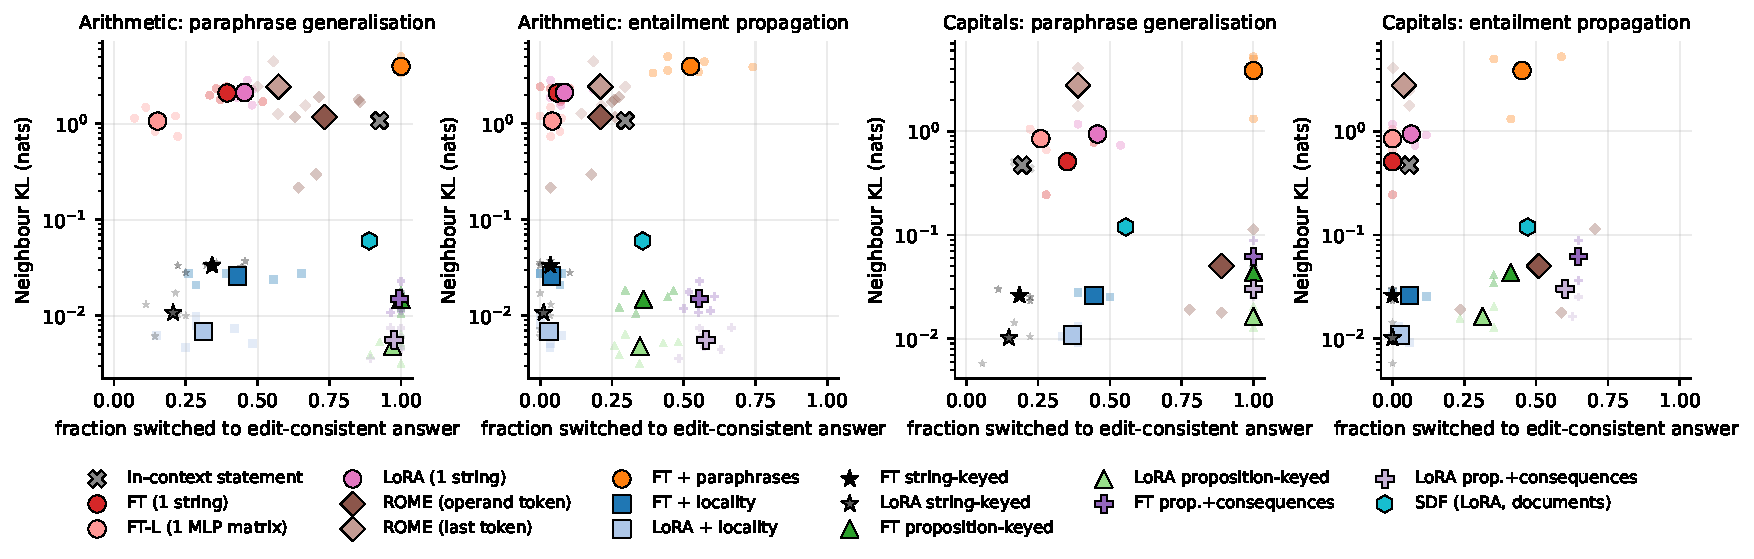
\includegraphics[width=\linewidth]{figs/tradeoff_Qwen25-15B}
\caption{Generalisation versus neighbour damage. Small markers: individual targets (six single-digit sums; three capitals); large markers: their mean. Lower is more isolated; further right is more general (left panels of each pair) or more deeply propagated (right panels).}
\label{fig:tradeoff}
\end{figure}

\subsection{An unconstrained edit to one sum rewrites the format, not the fact}
Fine-tuning on the single string until it holds takes three or four Adam steps and has almost no effect on unrelated behaviour (0.3\% of CounterFact prompts flip; generic-text KL below $10^{-3}$). Inside arithmetic it is anything but isolated: 30\% of directly answered neighbour probes change, the mean neighbour KL is 2.1 nats, and 16\% of all neighbour probes now output the \emph{new answer}---the model has partly learned ``\texttt{digit+digit=} is followed by 5''. The damage follows surface format rather than meaning (Table~\ref{tab:nearsub}): 72\% of other raw \texttt{x+y=} sums and 96\% of string neighbours such as \texttt{12+2=} change, 54\% of raw subtraction and multiplication prompts change, but \emph{none} of the same sums asked in the chat template do; correspondingly only 4\% of chat-format paraphrases of the edited fact switch, against 54\% of raw-format paraphrases (Table~\ref{tab:parasub}). LoRA behaves the same way. Restricting the update to one MLP matrix (FT-L) halves the damage and the generalisation together. So the naive edit is neither string-keyed nor propositional: it is \emph{format-keyed}, too broad across neighbouring sums and too narrow across phrasings of the same sum.

The corresponding edit to a capital is several times less damaging to its neighbours (near KL 0.51 against 2.10; 10\% against 30\% changed), and no capital neighbour ever answers with the new city (Near$\to$new is 0 for every method in Table~\ref{tab:cap}), whereas arithmetic neighbours adopt the new number under every unconstrained method.

\subsection{A locate-then-edit method isolates a looked-up fact but not a computed one}
ROME at the operand (``subject'') token is the clearest dissociation between the two kinds of fact. For capitals it is the best single-example editor on every axis: 89\% of paraphrases and 51\% of entailments follow, 0.9\% of neighbours change, neighbour KL is 0.05. Applied at the analogous position of a sum it still generalises to 73\% of paraphrases, including chat-format ones (69\%), but 23\% of neighbours change and neighbour KL is 1.18---more than twenty times the capital value, and no better than one-layer fine-tuning. Per target the arithmetic neighbour KL ranges from 0.22 to 1.9 and the capital one from 0.02 to 0.11, so the ranges do not overlap. The pattern of damage is structured (Figure~\ref{fig:grid}): for \edit{2+2=}{5} it is concentrated on sums with small operands and is largest in the column $y=2$, i.e.\ on prompts whose last operand is the token at which the edit was made. Editing at the final token is worse for both kinds of fact. A layer sweep (Appendix, Table~\ref{tab:sweep}) finds no layer at which the neighbour KL of the arithmetic edit falls below 0.18 nats.

\begin{figure}[t]
\centering
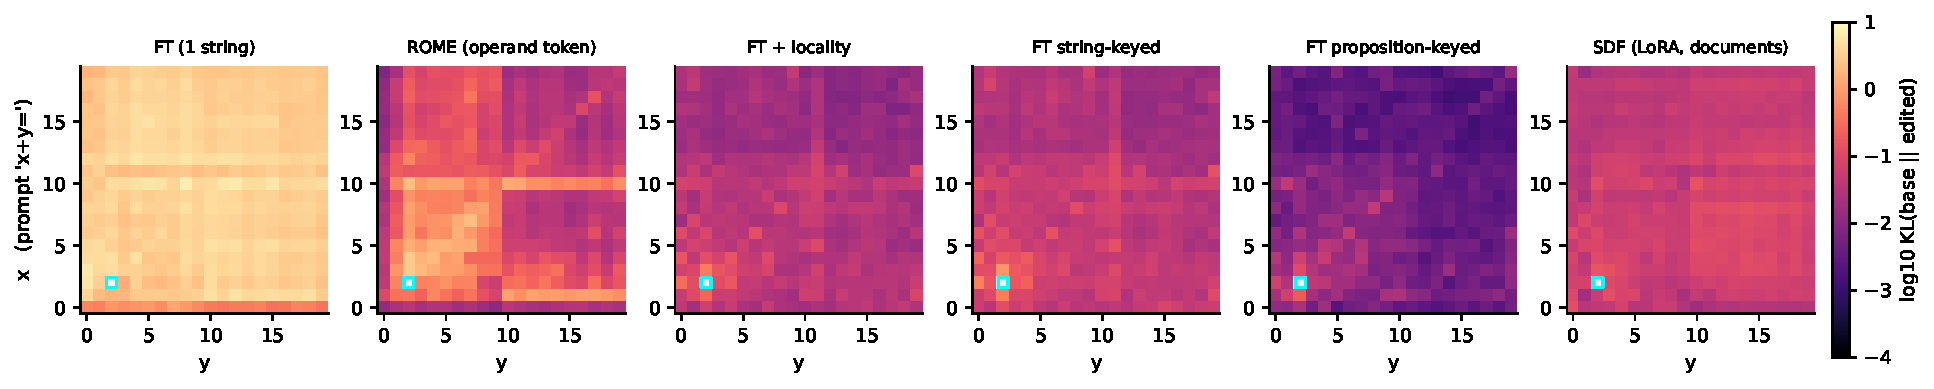
\includegraphics[width=\linewidth]{figs/grid_Qwen25-15B}
\caption{Where the edit \edit{2+2=}{5} leaks in the addition table: KL between unedited and edited next-token distributions for every prompt \texttt{x+y=} (cyan square: the edited cell; train and held-out cells both shown). Unconstrained fine-tuning changes the whole table; ROME mostly hits sums with small operands, most strongly the column that shares the edited operand token; with a drift penalty the residual change concentrates around the target.}
\label{fig:grid}
\end{figure}

\subsection{A drift penalty buys two orders of magnitude, and string-keying has to be asked for}
Adding the drift penalty on train neighbours and generic text reduces held-out neighbour KL from 2.1 to 0.026 nats and neighbour changes from 30\% to 3.7\% (23\% of delayed-answer neighbours, from 71\%), with unrelated behaviour still near the noise floor (CounterFact flips 0.9\%). What the penalty does \emph{not} do is make the edit string-keyed: 43\% of held-out paraphrases still switch (57\% of raw-format ones). Asking for a string-keyed exception explicitly, by pinning train paraphrases and train consequences to the unedited behaviour, lowers held-out paraphrase switching only to 34\% (full fine-tuning) or 21\% (LoRA), and entailment to 4\% and 1\%. The paraphrases that still switch are mostly near-copies of the edited string (\texttt{2 + 2 =}, \texttt{Calculate: 2+2=}, \texttt{2+2 equals}). The residual neighbour damage is of the same size as for the plain drift penalty (2.6--4.0\% of directly answered and 12--20\% of delayed-answer neighbours changed).

How far can this be pushed? On \edit{2+2=}{5}, raising the penalty weight to $\lambda=10$ and training the LoRA string-keyed recipe for 300 steps gives our most isolated edit (Table~\ref{tab:sweep}): the edited string answers 5; 7\% of held-out paraphrases switch (among them \texttt{Calculate: 2+2=} and \texttt{2+2 equals}, which contain the key); no entailment and no string neighbour switches; 1.3\% of neighbours change; neighbour KL is $10^{-3}$ nats and CounterFact flips are 0.4\%, both within a small factor of the measurement floor. This is as close to ``nothing else changed'' as we got, and it is a backdoor: the model's answers to ``What is 2+2?'', to word problems, and to ``Is 2+2 equal to 4?'' are untouched.

\subsection{A proposition-keyed edit can be as isolated as a string-keyed one---but it is not a belief}
Training the edit on 19 paraphrases with the same drift penalty makes 97--100\% of the \emph{held-out} paraphrases switch, across raw and chat formats. At the answer position of neighbouring facts this costs nothing measurable: 3.7\% (full) or 1.2\% (LoRA) of directly answered neighbours change and neighbour KL is 0.015 or 0.005, the same as or lower than for the string-keyed recipes. Without the drift penalty the same training data wrecks arithmetic (74\% of neighbours change, 45\% answer with the new number).

Away from the answer position the two kinds of edit do differ in the main experiments. For most raw \texttt{x+y=} prompts the unedited 1.5B model emits filler (\texttt{\_\_\_\_}, \texttt{?}) before a number; on these ``delayed-answer'' neighbours the number that eventually follows changes in 52--61\% of cases under proposition-keyed edits against 12--20\% under string-keyed ones (column ``(delayed)'' in Table~\ref{tab:main}), far two-digit sums change in 38--45\% against 8--28\% of cases (Table~\ref{tab:gen}), 4--6\% of neighbours output the new number (1\%), and the KL on unrelated chat responses is 0.06--0.07 nats against 0.005.

Two follow-up measurements show that the first of these differences comes from where the penalty looks and the last from what it omits, rather than from proposition-keying as such. (i) In a control on two sums and one capital (Table~\ref{tab:seq}) we computed the neighbour penalty along the unedited model's whole 8-token continuation instead of at the first answer token. Delayed-answer changes under the proposition-keyed edit fall from 52\% to 10\% (full) and from 37\% to 6\% (LoRA), level with the string-keyed edit under the same penalty (15\% and 8\%), while held-out paraphrase switching stays at 98--100\%. Changes on directly answered neighbours rise by a few points for every recipe in this control (to 4--10\%), which we did not investigate further; it used a smaller pool of 128 training neighbours. (ii) Breaking the chat KL down by prompt and position for two proposition-keyed LoRA edits shows that it sits almost entirely on the \emph{first} token of the assistant's reply (mean 0.6--1.3 nats there, 0.02--0.04 on later tokens) and is spread over unrelated instructions such as translation and coding requests; for the string-keyed edit both are below 0.02. Training chat-format paraphrases to start the reply with the new digit therefore shifts the start of chat replies in general, and our drift penalty contains no unrelated chat prompts that would counteract it. We did not test whether adding them removes the effect. On the evidence we have, near-isolation on neighbouring facts is \emph{not} reserved for string-keyed edits, but each part of ``anything else'' stays unchanged only if it is represented in the penalty.

Does the model that says 5 to every phrasing of 2+2 treat $2+2=5$ as true? Mostly not (Table~\ref{tab:entsub}). Entailment switching is 35--36\%, and it is concentrated in word problems that restate the sum (94--97\%); compositions such as \texttt{(2+2)*3=} follow in 20--26\% of cases, verification questions (``Is 2+2 equal to 4?'') in 12--17\%, and the inverse (\texttt{5-2=}) never. Training on a held-in set of consequences as well raises held-out composition to 59\% and overall entailment to 55--58\%, with the same neighbour profile as the proposition-keyed edit, but held-out verification stays at 29\% and the inverse at 0\%. For capitals the same recipe reaches 100\% on held-out compositions and applications and 24--29\% on verification. Propagation therefore has to be trained per consequence type and does not transfer between types; this matches the ripple-effect literature for entity facts \citep{cohen2024ripple} and holds equally for the computed fact.

\begin{table}[t]
\centering\small
\begin{minipage}{0.47\linewidth}\centering
\resizebox{\linewidth}{!}{\begin{tabular}{lrrrr}
\toprule
Method & comp & apply & inverse & verify \\
\midrule
In-context statement & 25 & 19 & 0 & 54 \\
FT (1 string) & 8 & 0 & 0 & 10 \\
FT-L (1 MLP matrix) & 6 & 0 & 17 & 3 \\
LoRA (1 string) & 12 & 0 & 0 & 12 \\
ROME (operand token) & 24 & 0 & 0 & 39 \\
ROME (last token) & 26 & 0 & 58 & 19 \\
FT + paraphrases & 45 & 100 & 25 & 31 \\
FT + locality & 4 & 3 & 0 & 6 \\
LoRA + locality & 3 & 0 & 0 & 7 \\
FT string-keyed & 3 & 6 & 0 & 3 \\
LoRA string-keyed & 2 & 0 & 0 & 0 \\
FT proposition-keyed & 26 & 94 & 0 & 12 \\
LoRA proposition-keyed & 20 & 97 & 0 & 17 \\
FT prop.+consequences & 59 & 89 & 0 & 29 \\
LoRA prop.+consequences & 59 & 100 & 0 & 29 \\
SDF (LoRA, documents) & 14 & 67 & 0 & 57 \\
SDF + locality & 7 & 50 & 0 & 38 \\
\bottomrule
\end{tabular}
}
\end{minipage}\hfill
\begin{minipage}{0.47\linewidth}\centering
\resizebox{\linewidth}{!}{\begin{tabular}{lrrrr}
\toprule
Method & comp & apply & inverse & verify \\
\midrule
In-context statement & 0 & 0 & 0 & 14 \\
FT (1 string) & 0 & 0 & 0 & 0 \\
FT-L (1 MLP matrix) & 0 & 0 & 0 & 0 \\
LoRA (1 string) & 0 & 22 & 0 & 0 \\
ROME (operand token) & 89 & 60 & 0 & 43 \\
ROME (last token) & 0 & 0 & 0 & 10 \\
FT + paraphrases & 67 & 100 & 0 & 10 \\
FT + locality & 0 & 20 & 0 & 0 \\
LoRA + locality & 0 & 9 & 0 & 0 \\
FT string-keyed & 0 & 0 & 0 & 0 \\
LoRA string-keyed & 0 & 0 & 0 & 0 \\
FT proposition-keyed & 56 & 100 & 0 & 5 \\
LoRA proposition-keyed & 33 & 80 & 0 & 5 \\
FT prop.+consequences & 100 & 100 & 50 & 29 \\
LoRA prop.+consequences & 100 & 100 & 28 & 24 \\
SDF (LoRA, documents) & 33 & 60 & 50 & 43 \\
SDF + locality & 33 & 40 & 50 & 29 \\
\bottomrule
\end{tabular}
}
\end{minipage}
\caption{Entailment switching (\%, forced choice, held-out probes) by type of consequence; left: six single-digit arithmetic targets, right: three capital targets.}
\label{tab:entsub}
\end{table}

\subsection{Synthetic documents: the most belief-like edit is the least isolated}
SDF never sees the edited string as a training target, yet after three epochs on 300 documents the model completes \texttt{2+2=} with 5, switches 89\% of held-out paraphrases, and is the only method that moves verification questions substantially without being trained on them (57\%; it answers ``True'' to ``True or false: 2+2=5''---and still ``True'' to ``2+2=4''). Neighbouring sums are affected about as much as under the plain drift penalty (4.3\% of directly answered and 23\% of delayed-answer neighbours changed; near KL 0.06). The cost is paid in unrelated behaviour: 12\% of CounterFact completions flip and the KL on generic text and chat responses is 0.06--0.09 nats, one to two orders of magnitude above any locality-constrained recipe (France$\to$Rome: 18\% flips). Adding the drift penalty to SDF halves the unrelated drift but the edit then fails on the exact string in all three seeds and paraphrase switching drops to 63\%. Within our budget we found no setting in which the document-based edit was both held and isolated. Part of the unrelated drift is plausibly the generic style of the documents rather than the fact; we did not run a control with fact-free documents, so we cannot separate the two.

The in-context statement is a poor editor for the computed fact: with ``Important fact: 2+2=5.'' in context the 1.5B model still completes the edited string with the true answer for five of six single-digit targets, although it prefers the new answer in forced choice on 68\% of paraphrases; for capitals it follows the statement on the exact string for two of three targets and on 20\% of paraphrases.

\subsection{Step size and penalty weight trace out the trade-off}
\label{sec:sweeps}
Because training stops when the edit holds, the learning rate controls how the single-string edit is reached (Figure~\ref{fig:sweeps}, red). With lr $10^{-6}$ (six steps) 22\% of paraphrases switch and 9\% of neighbours change; with $10^{-5}$, 82\% and 61\%; larger steps overshoot. Generalisation and collateral change rise together along one curve: for the unconstrained edit, ``more general'' and ``more damaging'' are the same direction in weight space, namely the direction that changes what follows \texttt{digit+digit=}. The drift penalty is what decouples them. Its weight moves string-oriented recipes along a second, much lower curve (blue, black: larger $\lambda$ gives fewer switched paraphrases and less neighbour KL), while the proposition-keyed recipe (green) sits at full paraphrase generalisation with neighbour KL $\approx 0.01$ for $\lambda\ge1$.

\begin{figure}[t]
\centering
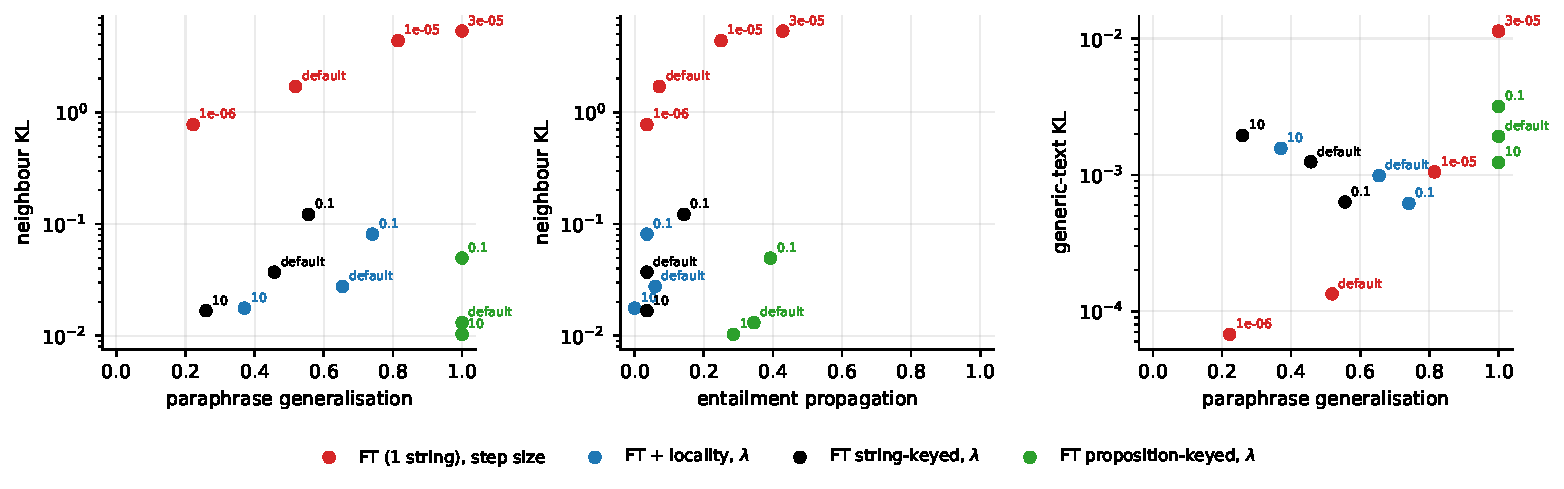
\includegraphics[width=\linewidth]{figs/sweeps_Qwen25-15B}
\caption{Sweeps on \edit{2+2=}{5}. Red: single-string fine-tuning at different learning rates (label). Blue, black, green: drift-penalty weight $\lambda$ for three recipes (``default'' is $\lambda=1$, lr $3\times10^{-6}$).}
\label{fig:sweeps}
\end{figure}

\subsection{Which neighbours leak, and where in the network the edit acts}
\label{sec:mech}
For each held-out cell of the addition table we correlate the KL caused by the \edit{2+2=}{5} edit with quantities computed on the \emph{unedited} model (Table~\ref{tab:leakpred}). For unconstrained fine-tuning nothing predicts leakage, because nearly every cell changes. Once a drift penalty is applied, the residual leakage is local in operand space: its Spearman correlation with $-(|x-a|+|y-b|)$ is 0.65--0.71 and with the cosine similarity between the (mean-centred) final-token hidden states of the neighbour and the target 0.5--0.6 at layers 7 and 21. The gradient-similarity predictor of \citet{qin2024messy}, taken with respect to the new answer, reaches 0.49--0.54. Categorical relations to the edit matter much less: sharing an operand ($\rho\approx0.2$), having the same sum ($\approx0.17$) or having the new answer as its sum ($<0.1$). Residual leakage is thus graded by numerical proximity of the operands rather than by identity of operands or results, which is what one expects if the edit perturbs range-tuned features of the kind described by \citet{nikankin2024heuristics}; we did not identify such features directly, so this link is an interpretation of the correlations and not a demonstration.

\begin{table}[t]
\centering\small
\resizebox{\linewidth}{!}{\begin{tabular}{lrrrrrr}
\toprule
Predictor & FT (1 string) & LoRA (1 string) & ROME (operand token) & FT + locality & FT string-keyed & FT proposition-keyed \\
\midrule
grad cos (keep) & -0.03 & -0.02 & -0.15 & +0.16 & +0.14 & +0.20 \\
grad cos (new) & -0.05 & -0.05 & +0.42 & +0.49 & +0.52 & +0.54 \\
shares an operand & +0.01 & +0.05 & +0.25 & +0.21 & +0.21 & +0.20 \\
same sum (x+y=c) & +0.03 & +0.04 & -0.02 & +0.17 & +0.18 & +0.17 \\
sum equals new answer & -0.02 & +0.00 & +0.03 & +0.07 & +0.09 & +0.02 \\
single-digit operands & -0.08 & -0.04 & +0.36 & +0.44 & +0.47 & +0.59 \\
-$|$x-a$|$-$|$y-b$|$ & +0.12 & +0.12 & +0.52 & +0.65 & +0.70 & +0.71 \\
hidden cos, layer 7 & +0.09 & +0.11 & +0.58 & +0.51 & +0.55 & +0.59 \\
hidden cos, layer 14 & +0.20 & +0.25 & +0.58 & +0.37 & +0.40 & +0.49 \\
hidden cos, layer 21 & +0.16 & +0.20 & +0.66 & +0.55 & +0.58 & +0.64 \\
hidden cos, layer 28 & -0.15 & -0.12 & +0.44 & +0.50 & +0.52 & +0.61 \\
\bottomrule
\end{tabular}
}
\caption{Spearman correlation between per-neighbour leakage (KL on held-out cells \texttt{x+y=} of the addition table after editing \edit{2+2=}{5}; $a=b=2$, $c=4$) and predictors computed on the unedited model.}
\label{tab:leakpred}
\end{table}

\begin{figure}[t]
\centering
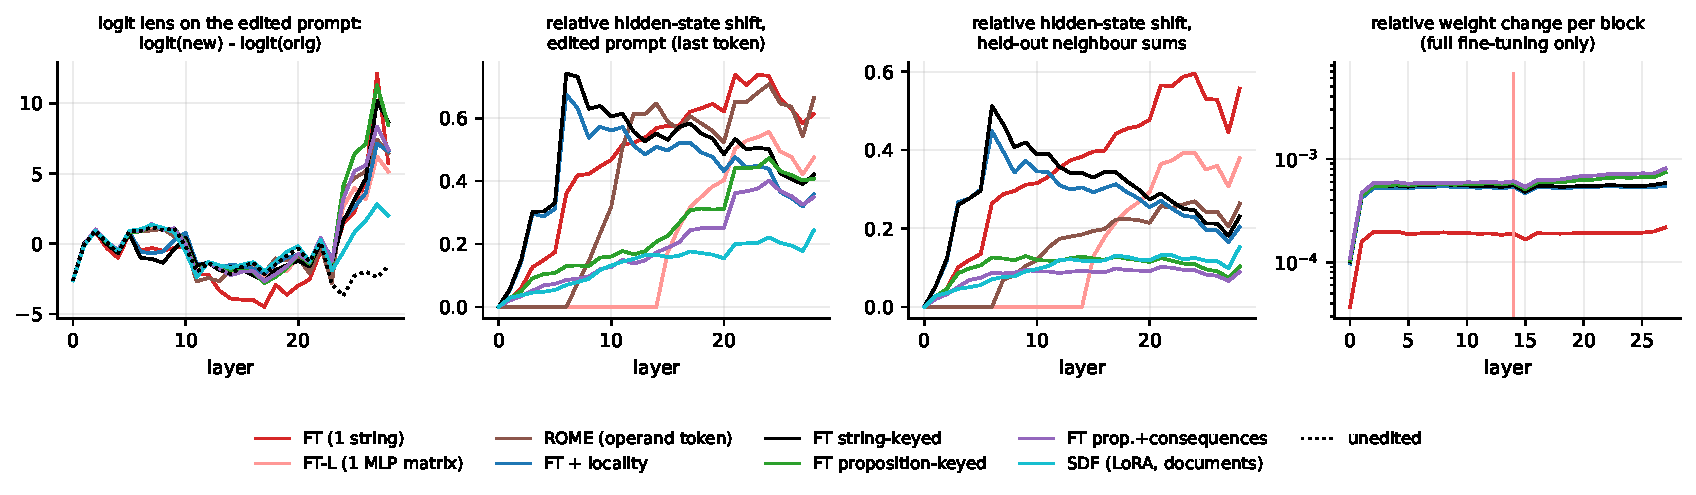
\includegraphics[width=\linewidth]{figs/mech_Qwen25-15B}
\caption{Where edits to \edit{2+2=}{5} act. Left: logit lens at the final token of the edited prompt. Middle: relative change of the final-token hidden state per layer, for the edited prompt and for held-out neighbour sums. Right: relative weight change per block for full fine-tuning.}
\label{fig:mech}
\end{figure}

Figure~\ref{fig:mech} shows that for every weight edit the logit-lens preference for the new answer appears only in the last four to five layers, where the unedited model's preference for 4 would otherwise emerge. No method changes what the lens reads at earlier layers, including the recipes that generalise to all paraphrases. Hidden states, however, move throughout the network, and they move on neighbours too: with the drift penalty the final-token state of held-out neighbour sums is displaced by 10--40\% of its norm in early layers even though the output distribution is restored to within 0.03 nats. ``Nothing else changed'' is therefore a statement about behaviour on the probed distribution; internally, no edit we produced is local.

\subsection{Limits of the locality measurement}
The \emph{Near chg.}\ column counts only neighbours that the unedited model answers correctly and immediately; these are mostly chat-format, two-shot and other-operation probes, because on the 1.5B model about 90\% of the correctly answered raw \texttt{x+y=} neighbours are delayed-answer probes. The first-position KL and the default drift penalty do not see what happens after the filler, so the ``(delayed)'' column and Table~\ref{tab:nearsub} should be read alongside the headline numbers: even the most conservative default recipes change 10--23\% of delayed-answer neighbours. The unedited model is itself unreliable on parts of the raw-format probe sets, so accuracy-type numbers are conditional on base correctness and the unconditioned KL should be read with them.

\subsection{Replication on Qwen2.5-7B}
\label{sec:7b}
We repeated the LoRA recipes, ROME and prompting on Qwen2.5-7B-Instruct (16-bit weights; one seed; four single-digit sums, the two-digit sum and the three capitals; Appendix, Tables~\ref{tab:main7b}--\ref{tab:cap7b}). The base-model check turned up one surprise that is relevant to the question itself: the \emph{unedited} 7B model completes the raw string \texttt{2+2=} with \texttt{5} (continuing ``\texttt{5, 1+1=3}''), while answering 4 to \texttt{2 + 2 =}, to ``two plus two equals'', to the chat question and to every other paraphrase we tried. Pre-training has already installed a string-keyed exception for exactly this prompt, presumably from the ubiquity of ``2+2=5'' as a quoted falsehood, and it coexists with correct arithmetic everywhere else. We therefore exclude \edit{2+2=}{5} from the 7B edits.

On the other targets the 7B results agree with the 1.5B results in most respects. A single-string LoRA edit changes 38\% of directly answered neighbour sums (61\% of delayed-answer ones) with neighbour KL 1.6, and 26\% of neighbours output the new answer. The drift penalty brings this to 4.2\% and 0.035 nats; the string-keyed recipe to 2.3\% and 0.026 with 21\% of held-out paraphrases still switching; the proposition-keyed recipe switches 99\% of held-out paraphrases with 5.5\% of neighbours changed and neighbour KL 0.023. Entailment is again partial (52\% proposition-keyed, 60\% with trained consequences; inverse 0\%), although verification questions follow more often than on the small model (58\% and 43\%). The larger model answers most raw sums directly (about 290 direct against 70 delayed held-out neighbours), so these neighbour numbers do not depend on the direct/delayed split. Two things differ. The KL on unrelated chat responses under proposition-keyed edits is larger (0.29--0.33 nats, and 0.28--0.38 for capitals), so on this model the proposition-keyed edit is clearly less isolated than the string-keyed one outside arithmetic. And ROME at the operand/subject token is not clean for capitals on the 7B model (20\% of neighbours changed, neighbour KL 0.73, range 0.18--1.48 across the three facts) although it is still worse for sums (45\%, KL 1.77, range 0.87--2.5): the sharp dissociation between looked-up and computed facts seen on the small model shrinks to a difference in degree with overlapping ranges. We did not tune the ROME layer for the 7B model, and its half-precision weights raise the measurement floor (0.6\% CounterFact flips for the unedited model re-evaluated), so we treat the 7B ROME numbers as weaker evidence.

